\noindent \scalebox{0.8}{\textit{Reference: \cite{zumstein2021}}}
\smallskip

Excel (or Google Sheets) is unavoidable if you work with enough people, especially ThinkPad people. You will want to deliver a spreadsheet to a stakeholder, not a Python script. And that spreadsheet will be received better if it's well formatted. That means we're not talking about a CSV file fresh from \code{df.to_csv()}. In this chapter, we'll use Python to do the following.

\begin{enumerate}
    \item Save to individual sheets in a larger workbook.
    \item Read in individual sheets as dataframes.
    \item Apply cell formatting.
    \item Apply filters.
    \item Insert plots in a sheet.
\end{enumerate}

\noindent If you're in this class, you're way too smart to do these tasks by pointing and clicking in a GUI. We'll use pandas and \link{https://openpyxl.readthedocs.io/en/stable/}{OpenPyXL}.% and \link{https://xlsxwriter.readthedocs.io/}{XlsxWriter}. 

\section{Pandas}

Pandas comes with the \code{read_excel()} function and the \code{to_excel()} method. Below, we use these most basically. 

\begin{lstlisting}
df = pd.DataFrame({'a': [0]})

# Save to excel file
df.to_excel("mwe.xlsx", index = None)

# Clear df from memory
del df

# Read
df = pd.read_excel("mwe.xlsx")
\end{lstlisting}

We go into more detail in this section. However, pandas is limited. Separate reader and writer packages are useful for including charts, changing formatting, etc. 

\subsection{Reading}

Above, \texttt{mwe.xlsx} is the simplest and most well-behaved kind of Excel file you can encounter. There are not multiple sheets and the data begins in cell A1. Often, you'll receive an Excel file with multiple sheets and with some formatting that, to a Python user, is wonky. Reading in the right sheets is priority number one. You can use the \code{sheet_name} parameter to specify the sheet you want to use, by name or index. If you pass a list of sheet names, \code{read_excel()} returns a dictionary with the DataFrames as values and sheet names as the keys. Use \code{sheet_name = None} to load all of the sheets. 

Maybe the first row and first column are blank, in which case the data begins in cell B2. 
Use \code{skiprows} and \code{usecols} to specify the cell range you want to use. These and other parameters are described in Table 7-1 in \cite{zumstein2021}. The additional parameters are mostly useful for data cleaning, so you can have that done in the \code{read_excel()} call instead of in additional lines of code. 

\subsection{Writing}

As with \code{read_excel()}, \code{to_excel()} includes a \code{sheet_name} parameter. However, this can't be used to add multiple sheets to a single Excel file. The method doesn't \emph{add} a new sheet to an existing file, it merely writes the Excel file from scratch, with a single sheet named according to \code{sheet_name}. 

\begin{lstlisting}
df = pd.DataFrame({'a': [0]})

# creates mwe.xlsx with one sheet called A
df.to_excel("mwe.xlsx", index = None, sheet_name = 'A')

# overwrites mwe.xlsx, one sheet called B
df.to_excel("mwe.xlsx", index = None, sheet_name = 'B')
\end{lstlisting}


To add multiple DatFrames to different sheets (or even within the same sheet), you need to use the \code{ExcelWriter} class. Below, we use \code{ExcelWriter} as a \emph{context manager}, using a \code{with} statement. 

\begin{lstlisting}
df_a = pd.DataFrame({'a': [0]})
df_b = pd.DataFrame({'b': [1]})

with pd.ExcelWriter('multi_sheet.xlsx') as writer:
    df_a.to_excel(writer, sheet_name = 'A', index = None)
    df_b.to_excel(writer, sheet_name = 'B', index = None)
\end{lstlisting}

The additional parameters for \code{to_excel()} deserve some attention, because they aren't as easily replaced by other lines of code. Neglecting them creates more work for you in Excel, and our objective is to avoid that. Some parameters are described in Table 7-2 in \cite{zumstein2021} and in the \link{https://pandas.pydata.org/docs/reference/api/pandas.DataFrame.to_excel.html}{official documentation}. 

\begin{center}
\begin{small}
{\setlength{\tabcolsep}{2em}
\begin{tabular}{ll}
\toprule
Parameter & Description \\
\midrule
\code{startrow} & First row where the DataFrame is written (using zero-based indexing) \\
\code{startcol} & First column where the DataFrame is written (using zero-based indexing) \\
\code{freeze_panes} & Takes a tuple for the number of rows and columns to freeze. \\
& Passing \code{(1,2)} freezes the first row and the first two columns. \\
\bottomrule
\end{tabular}}
\end{small}
\end{center}

\section{OpenPyXL}

\paragraph{Installation:}
OpenPyXL is useful for reading, writing, and editing Excel files. If you need to install it, run \texttt{conda install -c anaconda openpyxl} or \texttt{pip install openpyxl} in the terminal. %We'll also need Pillow to include images. Thus, \texttt{conda install -c anaconda pillow} or \texttt{pip install pillow}.

Remember, there are three levels to an Excel file: the workbook, the worksheet, and the individual cells. The workbook is the entire file and all the sheets (or tabs). The worksheet is an individual tab. And a cell is the entry at a specific coordinate in a worksheet. OpenPyXL has classes \code{Workbook}, \code{Worksheet}, and \code{Cell} for each of these. 

\subsection{Reading}

Use \code{load_workbook()} to read in data and specify \code{data_only = True} to read in the cell values instead of the cell formulas.

\begin{lstlisting}
import pandas as pd
import openpyxl
import datetime as dt

# Workbook object
book = openpyxl.load_workbook('multi_sheet.xlsx', data_only = True)

# get a list of all sheet names
print(book.sheetnames)

# Worksheet objects
sheet_a = book['A']
sheet_b = book['B']

# Get dimensions
print(sheet_a.max_row, sheet_a.max_column)

# Cell object
cell = sheet_a['A1']
print(cell.value)
\end{lstlisting}

\subsection{Writing}


We write a DataFrame to an Excel .xlsx file using the functionality provided directly in OpenPyXL, making use of \code{dataframe_to_rows}.\footnote{\cite{zumstein2021} provides a module \link{https://github.com/fzumstein/python-for-excel/blob/1st-edition/excel.py}{excel.py}. It's handy for going back and forth between OpenPyXL and other Excel packages. However, it doesn't play that well with index and header values.} The process is as follows. 

\begin{enumerate}
    \item Create a Workbook instance.
    \item Access a Worksheet. Below we use the \code{active} attribute to get the currently active sheet.
    \item Append data to the bottom of the sheet using the Worksheet \code{append()} method. 
    \item Save the Workbook using the \code{save()} method.
\end{enumerate}

\begin{lstlisting}
from openpyxl.utils.dataframe import dataframe_to_rows

wb = openpyxl.Workbook()
ws = wb.active

for r in dataframe_to_rows(df, index=True, header=True):
    ws.append(r)

wb.save("pandas_openpyxl.xlsx")
\end{lstlisting}

This includes the index and header (column name) values given the parameters in \code{dataframe_to_rows}. Our Excel file includes a sheet as shown below. 

\begin{center}
    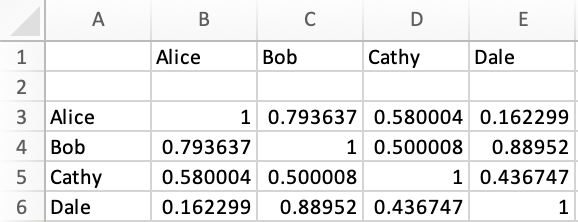
\includegraphics[width = 0.7\textwidth]{images/excel_ss1.png}
\end{center}

\noindent If we had simply used \code{df.to_excel('filename.xlsx')}, we'd end up with the below. 

\begin{center}
    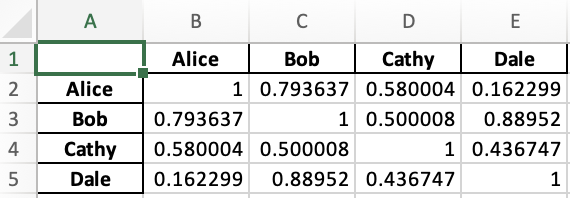
\includegraphics[width = .7\textwidth]{images/excel_pandas_save.png}
\end{center}

\noindent Why the empty row when using OpenPyXL? I'm not sure.\footnote{See the \link{https://openpyxl.readthedocs.io/en/stable/pandas.html?highlight=dataframe\#working-with-pandas-dataframes}{documentation here} if you'd like to delve further on your own.} The \code{dataframe_to_rows()} function finds an empty row somewhere, somehow. We can avoid appending this to our worksheet by modifying the for-loop, as is done below. 

\begin{lstlisting}[label = {lst:wb}]
from openpyxl.utils.dataframe import dataframe_to_rows

wb = openpyxl.Workbook()
ws = wb.active

for r in dataframe_to_rows(df, index=True, header=True):
    print(r)
    if r != [None]:
        ws.append(r)

wb.save("pandas_openpyxl.xlsx")
\end{lstlisting}


\subsection{Styles}

Styles and formatting can be applied, but only one cell at a time. Accordingly, we need to learn more about the \code{Cell} class.\footnote{\link{https://openpyxl.readthedocs.io/en/stable/api/openpyxl.cell.cell.html}{\code{Cell} documentation here.}} A specific cell can be accessed by indexing a worksheet with the appropriate coordinate, \code{ws['A1']} for example. Cell ranges can be accessed as might be done in Excel. Columns A-C can be obtained with \code{ws['A:C']}. Rows 3-5 can be accessed with \code{ws[3:5]}. Note cell ranges are just tuples of cells. There is also a \code{iter_rows()} worksheet method, returning a generator for iteration. 

Below are some basic \code{Cell} attributes.

\begin{center}
\begin{small}
{\setlength{\tabcolsep}{2em}
\begin{tabular}{ll}
\toprule
Attribute & Description \\
\midrule
\code{coordinate} & The Excel coordinate of the cell (e.g. \code{'B2'}) \\
\code{column} & Column number of the cell (one-based) \\
\code{row} & Row number of the cell (one-based) \\
\code{column_letter} & Column letter of the cell (e.g. \code{'B'} or \code{'AA'}) \\
\code{value} & Data value of the cell \\
\code{is_date} & Boolean value \\
\bottomrule
\end{tabular}}
\end{small}
\end{center}

There are \code{Cell} style attributes you might use to inspect and to overwrite the cell font, border, alignment, fill, and number format. To set these, use the \code{openpyxl.styles} submodules. For example, to set the cell alignment, write \code{ws['C8'].alignment = openpyxl.styles.alignment.Alignment(horizontal = 'center')}.

\begin{center}
\begin{small}
{\setlength{\tabcolsep}{2em}
\begin{tabular}{ll}
\toprule
Attribute & \code{openpyxl.styles} submodule and class  \\
\midrule
\code{font} & \code{Font} \\
\code{border} & \code{borders.Side} and \code{borders.Border} \\
\code{alignment} & \code{alignment.Alignment} \\
\code{fill} & \code{fills.PatternFill} \\
\code{number_format} & N/A (use a string) \\
\bottomrule
\end{tabular}}
\end{small}
\end{center}

The final attribute listed above, \code{number_format}, is set with a string. Available format examples can be found in the \link{https://openpyxl.readthedocs.io/en/stable/_modules/openpyxl/styles/numbers.html}{OpenPyXL documentation} and the \link{https://support.microsoft.com/en-us/office/review-guidelines-for-customizing-a-number-format-c0a1d1fa-d3f4-4018-96b7-9c9354dd99f5}{Microsoft documentation} provides further detail. Below are a few formats and their Excel output.\footnote{Access the \link{https://docs.google.com/spreadsheets/d/10ME-F1CMkeUCXRyoUj3EYsKFvfyyJe61/edit?usp=sharing&ouid=102598671780190894865&rtpof=true&sd=true}{spreadsheet here}.}


\begin{center}
    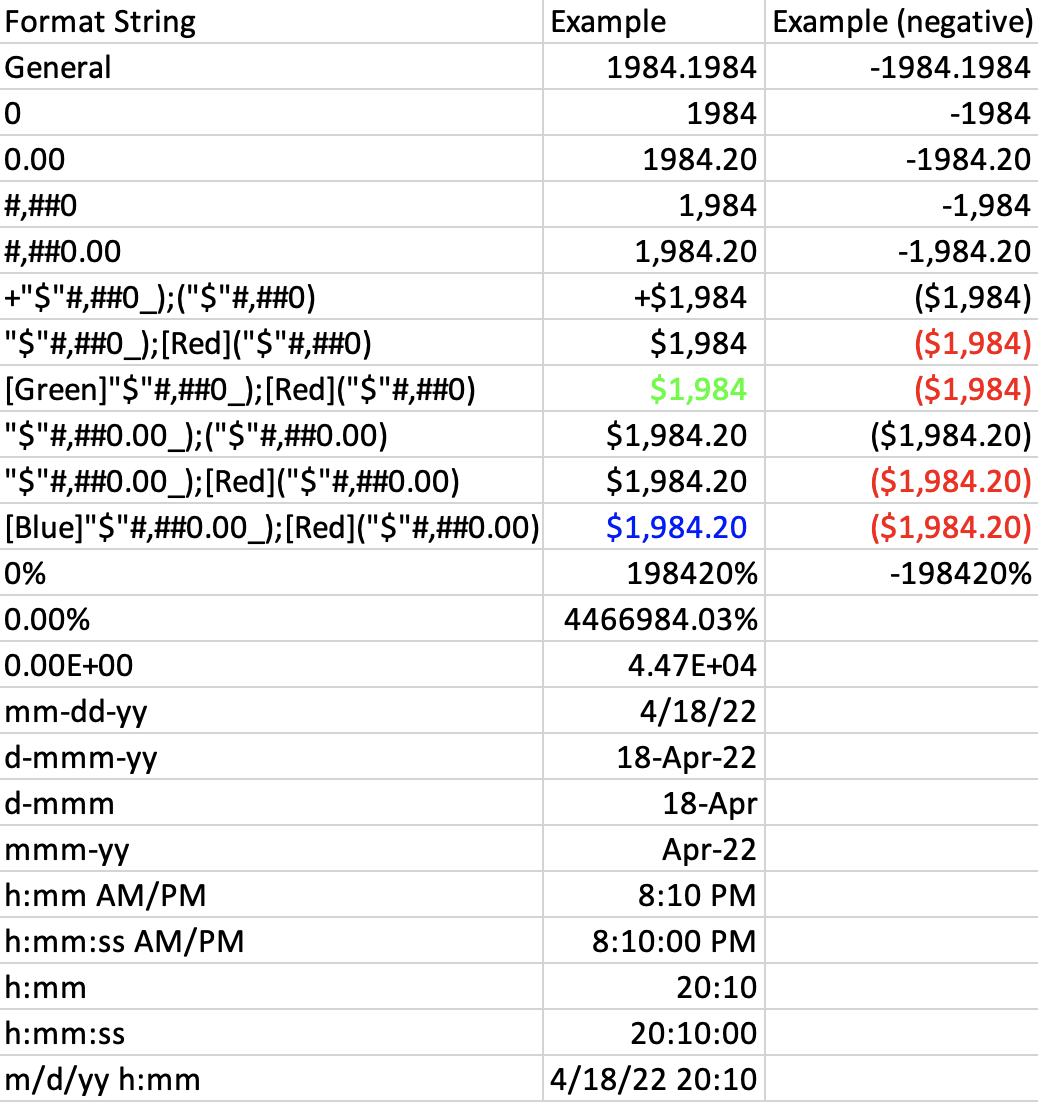
\includegraphics[width = .8\textwidth]{images/excel_formats2.png}
\end{center}

The above is created with this code. 

\begin{lstlisting}
import openpyxl

formats = ['General',
     '0',
     '0.00',
     '#,##0',
     '#,##0.00',
     '+"$"#,##0_);("$"#,##0)',
     '"$"#,##0_);[Red]("$"#,##0)',
     '[Green]"$"#,##0_);[Red]("$"#,##0)',
     '"$"#,##0.00_);("$"#,##0.00)',
     '"$"#,##0.00_);[Red]("$"#,##0.00)',
     '[Blue]"$"#,##0.00_);[Red]("$"#,##0.00)',
     '0%',
     '0.00%',
     '0.00E+00',
     'mm-dd-yy',
     'd-mmm-yy',
     'd-mmm',
     'mmm-yy',
     'h:mm AM/PM',
     'h:mm:ss AM/PM',
     'h:mm',
     'h:mm:ss',
     'm/d/yy h:mm']

wb = openpyxl.Workbook()
ws = wb.active

ws['A1'] = 'Format String'
ws['B1'] = 'Example'
ws['C1'] = 'Example (negative)'
for key, fmt in enumerate(formats):
    
    coord1 = 'A{}'.format(key + 2)
    coord2 = 'B{}'.format(key + 2)
    coord3 = 'C{}'.format(key + 2)
    
    # plain format string
    ws[coord1].value = fmt
    
    # set a date or numeric value and apply format
    if key > 11:
        ws[coord2].value = dt.datetime(2022,4,18,20,10)
    else:
        ws[coord2].value = 1984.1984
        ws[coord3].value = -1984.1984
        ws[coord3].number_format = fmt
    ws[coord2].number_format = fmt

wb.save("openpyxl_formats.xlsx")
\end{lstlisting}

\noindent This leaves \link{https://openpyxl.readthedocs.io/en/stable/api/openpyxl.styles.fonts.html?highlight=fonts\#openpyxl.styles.fonts.Font}{fonts}, \link{https://openpyxl.readthedocs.io/en/stable/api/openpyxl.styles.borders.html?highlight=border\#openpyxl.styles.borders.Border}{borders}, \link{https://openpyxl.readthedocs.io/en/stable/api/openpyxl.styles.alignment.html?highlight=alignment\#openpyxl.styles.alignment.Alignment}{alignment}, and \link{https://openpyxl.readthedocs.io/en/stable/api/openpyxl.styles.fills.html?highlight=patternfill\#module-openpyxl.styles.fills}{fills} to be explored. 

Here is an example with the Excel result further below. 

\begin{lstlisting}
import openpyxl
import openpyxl.styles as osty
wb = openpyxl.Workbook()
ws = wb.active

words = 'My cup runneth over.'.split(" ")
letters = 'ABCD'
for l, s in zip(letters, words):
    ws['{}1'.format(l)].value = s
    
ws['A1'].font = osty.Font('Times New Roman', bold = True, color = '006400')

ws['B1'].alignment = osty.alignment.Alignment(horizontal = 'right', 
                                              vertical = 'top', 
                                              textRotation = 30)

ws['C1'].fill = osty.fills.PatternFill(fgColor = 'FFFFE3', 
                                       fill_type = 'solid')

medium = osty.borders.Side(border_style = 'medium',
                           color = 'FF0000')
dotted = osty.borders.Side(border_style = 'dotted',
                           color = '87E0FF')
ws['D1'].border = osty.borders.Border(top = medium, 
                                         bottom = medium,
                                         left = dotted,
                                         right = dotted)

wb.save("openpyxl_cup.xlsx")
\end{lstlisting}


\begin{center}
    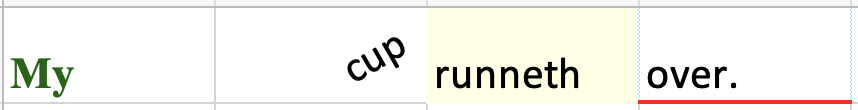
\includegraphics[width = .58\textwidth]{images/cup_runneth.png}
\end{center}

The above uses \code{PatternFill}. There's also \code{GradientFill}, used below. I'm not sure anyone has a use for it. Nonetheless: 

\begin{lstlisting}
wb = openpyxl.Workbook()
ws = wb.active

strings = ['Every man is important if he loses his life;',
         'and every many is funny if he loses his hat and has to run after it.']

for key, s in enumerate(strings):
    ws['A{}'.format(key+1)].value = s

for cell in ws['A']:
    cell.font = osty.Font('Times New Roman', bold = True)

ws['A1'].fill = osty.fills.GradientFill(stop = ['1D97C1', 'FFFFFF'])
ws['A2'].fill = osty.fills.GradientFill(stop = ['FFFFFF', '008080'], degree = 90)

wb.save("openpyxl_chesterton.xlsx")
\end{lstlisting}

\begin{center}
    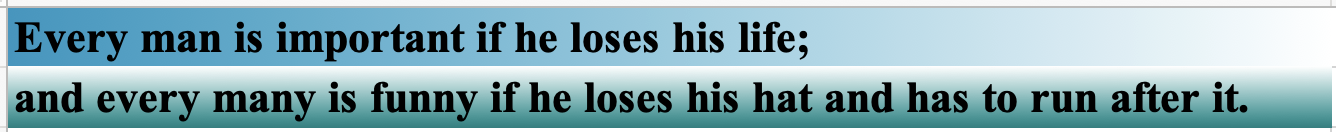
\includegraphics[width = .8\textwidth]{images/excel_chesterton.png}
\end{center}

\subsubsection{Conditional Formatting and Filtering}

Next, we consider conditional formatting. In my experience, the vast majority of any Excel formatting I did was applying a filter and conditional formatting. Below, we take a DataFrame with cosine similarities and send it to a formatted Excel file. 

\begin{lstlisting}
from openpyxl.formatting.rule import ColorScaleRule
import numpy as np
np.random.seed(1)

# Data Generation
a = np.random.rand(n, n)
a = np.triu(a, k = 1) + np.triu(a).T
similarities = a - np.diag(np.diag(a)) + np.diag(np.ones(n))

# Send to DataFrame with index and headers
names = ['product{:0>2}'.format(x) for x in range(n)]
df = pd.DataFrame(similarities, index = names, columns = names)

# Create book and sheet
book = openpyxl.Workbook()
ws = book.active
ws.title = 'Product Similarities'

# Send data to worksheet
for r in dataframe_to_rows(df, index=True, header=True):
    if r != [None]:
        ws.append(r)
        
# Create and apply color rule
rule = ColorScaleRule(start_type='percentile', start_value=10, start_color='ea9999', # red
                       mid_type='percentile', mid_value=50, mid_color='FFFFFF', # white 
                       end_type='percentile', end_value=90, end_color='b6d7a8') # green
ws.conditional_formatting.add('A1:AP42', rule)

# Add Filter over entire spreadsheet
ws.auto_filter.ref = ws.calculate_dimension()

book.save("similarities.xlsx")
\end{lstlisting}


\begin{center}
    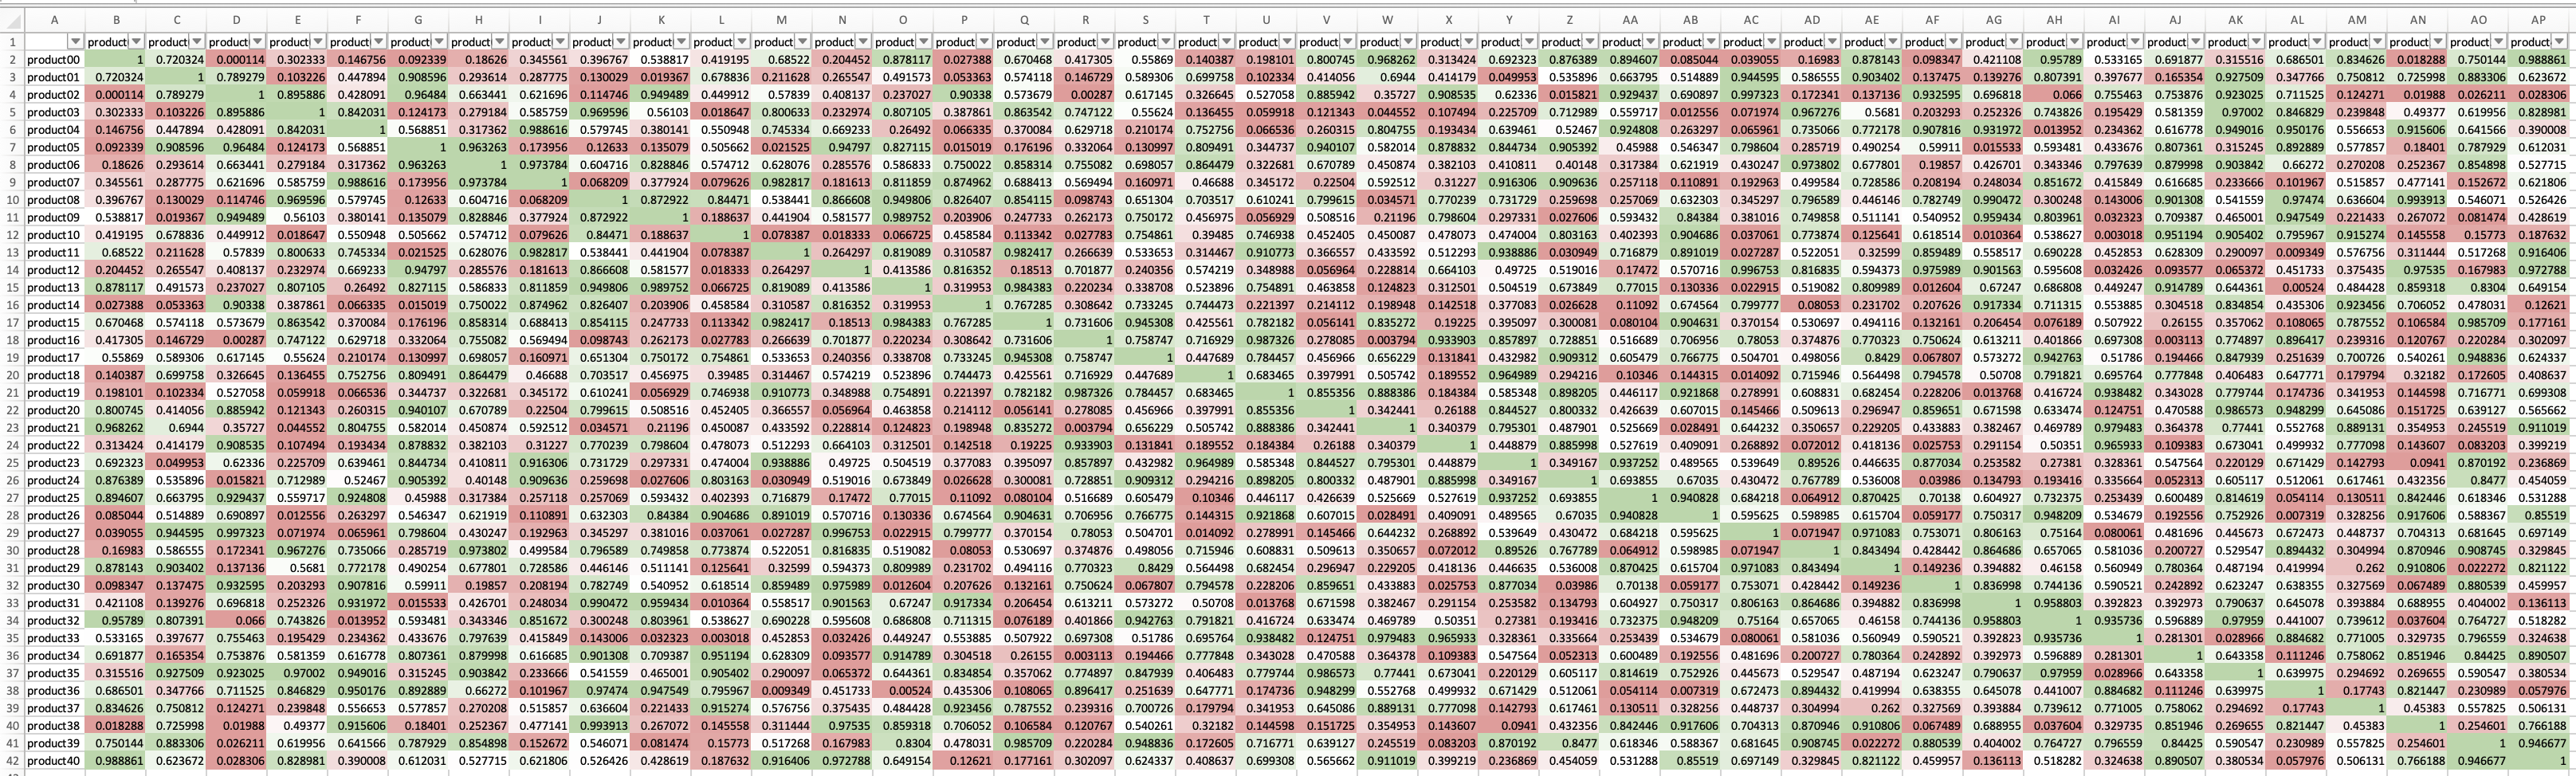
\includegraphics[width = .95\textwidth]{images/similarities.png}
\end{center}



\subsection{Inserting Charts}

Next, we'll add a bar chart using OpenPyXL. See \cite{zumstein2021} Chapter 9 for adding matplotlib images to an Excel file. It's better to include an actual Excel chart as the Excel file user can make further modifications. 



\begin{lstlisting}
#https://openpyxl.readthedocs.io/en/latest/charts/bar.html
from openpyxl import Workbook
from openpyxl.chart import BarChart, Reference

wb = Workbook(write_only=True)
ws = wb.create_sheet()

rows = [ 
        ["Program", 'Wins'],
        ['Kansas', 2357],
       ['Kentucky', 2353],
       ['North Carolina', 2323],
       ['Duke', 2246] ]

for row in rows: #bball_data.reset_index().to_numpy():
    ws.append(row)


chart = BarChart(varyColors = True)
chart.type = "col"
#chart.style = 11
chart.title = "Programs with Most Wins (NCAA Men's Basketball)"
chart.y_axis.title = 'Wins'
chart.x_axis.title = 'Program'

chart.legend = None
data = Reference(ws, min_col=2, min_row=1, max_row=5, max_col=2)
cats = Reference(ws, min_col=1, min_row=2, max_row=5)

chart.add_data(data, titles_from_data=True)
chart.set_categories(cats)

ws.add_chart(chart, "D4")

wb.save("basketball.xlsx")
\end{lstlisting}


We get output like this. 

\begin{center}
    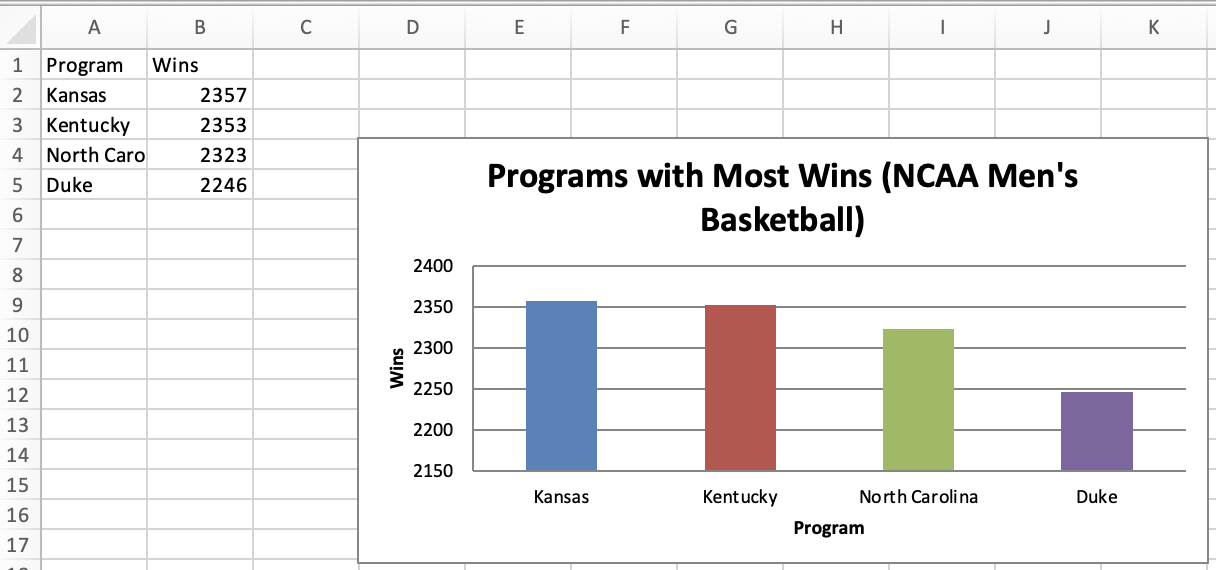
\includegraphics[width = .8\textwidth]{images/basketball_excel.png}
\end{center}